
\usetikzlibrary{calc}

\def\valA{30}
\def\valCA{0.3}
\def\valCB{0.7}
\def\valEA{0.2}
\def\valT{0}
\newcommand{\freeEnergy}[1]{\valA*((#1-\valCA)^2 * (#1-\valCB)^2) + (#1) * \valEA }
\newcommand{\freeEnergyP}[1]{2*\valA*((#1-\valCA)^2 * (#1-\valCB) + (#1-\valCA) * (#1-\valCB)^2) + \valEA }


\newcommand{\slope}[2]{(\freeEnergy{#1} - \freeEnergy{#2})/(#1-#2)}
\newcommand{\corde}[3]{\freeEnergy{#3} + (\freeEnergy{#2} - \freeEnergy{#3}) * (#1-#3)/(#2-#3)}
\newcommand{\tangent}[2]{\freeEnergy{#2} + \freeEnergyP{#2} * (#1-#2)}

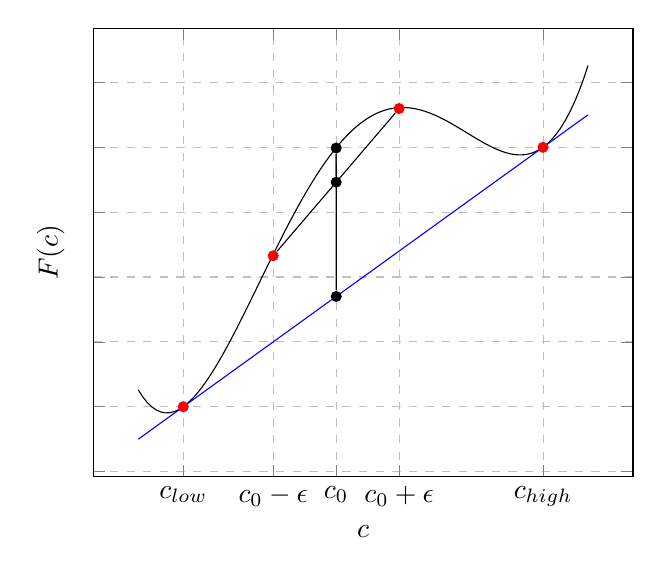
\begin{tikzpicture}

\def\cm{0.47}
\def\eps{0.07}
\pgfmathsetmacro{\cg}{\cm-\eps}
\pgfmathsetmacro{\cd}{\cm+\eps}


\begin{axis}[
% width=300pt,
%axis lines = left,
xlabel = \(c\),
ylabel = {\(F(c)\)},
xmajorgrids=true,
ymajorgrids=true,
scaled ticks=false,
% xticklabel=\empty,
yticklabel=\empty,
xtick={\valCA,\cg,\cm,\cd,\valCB},
% extra x tick style={grid=none},
xticklabels={%
{$c_{low}$},
{$c_0-\epsilon$},
{$c_0$},
{$c_0+\epsilon$},
{$c_{high}$}
},
grid style=dashed,
] % end axis options




\addplot[
domain=0.25:0.75,
samples=100,
color=black
]% end plot options
{\freeEnergy{x}};


\addplot[
domain=0.25:0.75,
samples=100,
color=blue,
]% end plot options
{\tangent{x}{\valCB}};


\pgfmathsetmacro{\vg}{\freeEnergy{\cg}}
\node[fill,circle,inner sep=0,minimum size=4pt,color=red] (cgf) at (axis cs:\cg,\vg) {};
\pgfmathsetmacro{\vd}{\freeEnergy{\cd}}
\node[fill,circle,inner sep=0,minimum size=4pt,color=red] (cdf) at (axis cs:\cd,\vd) {};
\pgfmathsetmacro{\vm}{\freeEnergy{\cm}}
\node[fill,circle,inner sep=0,minimum size=4pt] (cmf) at (axis cs:\cm,\vm) {};
\node[fill,circle,inner sep=0,minimum size=4pt] (cepsf) at ($(cgf)!0.5!(cdf)$) {};

\draw (cgf) -- (cdf);
\draw (cmf) -- (cepsf);



\pgfmathsetmacro{\vgt}{\freeEnergy{\valCA}}
\node[fill,circle,inner sep=0,minimum size=4pt,color=red] (cgt) at (axis cs:\valCA,\vgt) {};
\pgfmathsetmacro{\vdt}{\freeEnergy{\valCB}}
\node[fill,circle,inner sep=0,minimum size=4pt,color=red] (cdt) at (axis cs:\valCB,\vdt) {};

\node[fill,circle,inner sep=0,minimum size=4pt] (cmt) at (intersection of cgt--cdt and cmf--cepsf) {};

\draw (cmf) -- (cmt);
% \draw (cmf) -- ($(cmf)+(1,0)$);


\end{axis}



\end{tikzpicture}

